%%%%%%%%%%%%%%%%%%%%%%%%%%%%%%%%%%%%%%%%%%%%%%%%%
%------ LaTeX-Template für Abschlussarbeiten, Prof. Thomas Görne, Dezember 2012 --------
%------ Modified by B.Sc. Julius Neudecker, May 2021 ------
%%%%%%%%%%%%%%%%%%%%%%%%%%%%%%%%%%%%%%%%%%%%%%%%%

%---- Header (mit Formateinstellugen) laden, Inputencoding prxfen ------

%%%%%%%%%%%%%%%%%%%%%%%%%%%%%%%%%%%%%%%%%%%%%%%%%
%---- LaTeX-Header fuer Abschlussarbeiten, Prof. Thomas Goerne, Dez. 2012/Aug. 2013 ----
%------ Modified by B.Sc. Julius Neudecker, May 2021 ------
%%%%%%%%%%%%%%%%%%%%%%%%%%%%%%%%%%%%%%%%%%%%%%%%%

\documentclass[12pt,paper=A4,pointlessnumbers,bibtotoc,liststotoc,DIV=11,BCOR=1mm]{scrreprt}
% BCOR ist die Bindekorrektur (verlorener Rand am linken Blattrand)! Wert haengt von der Art der Heftung ab!!
% DIV ist eine Satzspiegeleinstellung von KOMA-Script / sccreprt.

\pagestyle{headings}

\usepackage[T1]{fontenc} % Font Encoding fuer europaeische Schriften mit Umlauten (Unterstuetzung der Worttrennung)
\usepackage{lmodern} % PostScript-Varianten der TeX Computer Modern-Schriften laden
\usepackage[english]{babel} % Spracheinstellungen fuer Englisch und Neudeutsch laden

\usepackage{graphicx} % Grafikeinbindung (fuer .JPG, .JPEG, .PNG und .PDF, falls pdflatex benutzt wird)
\usepackage[table]{xcolor} % ermoeglicht farbige Schrift und farbige Tabellenzeilen
\definecolor{black}{gray}{0} % Umdefinition der Farbe black, falls noetig (0=schwarz, 1=weiss)
\definecolor{dblue}{rgb}{0.1,0.2,0.6} % Dunkelblau, fuer Hyperlinks
\definecolor{lgray}{gray}{0.9} % Hellgrau, fuer Tabellen (0=schwarz, 1=weiss)

\usepackage{booktabs} % fuer schoene Tabellen

\usepackage[round,authoryear]{natbib} % Literaturverweise mit Name/Jahreszahl in runden Klammern
\bibpunct[:\,]{(}{)}{,}{a}{}{,~}  % Feinformatierung der Natbib-Zitierweise

\usepackage[hyphens]{url}
\usepackage[colorlinks=true,linkcolor=black,citecolor=dblue,urlcolor=dblue]{hyperref} 
\usepackage{hyperref}  
% die Pakete url und hyperref ermoeglichen anklickbare URLs im Quellenverzeichnis in definierter Farbe, 
% sie ermoeglichen den Zeilenumbruch bei langen URLs, und sie erzeugen Hyperlinks (Farbe s.o.) 
% zwischen Quellenverweis und Quellenverzeichnis sowie zwischen label und ref im PDF-Dokument

% Fonteinstellungen fuer Bildunterschriften: Unterschrift serifenlos, "Abbildung" fett (bfseries = bold face series)
\setkomafont{captionlabel}{\sffamily\bfseries}
\setkomafont{caption}{\sffamily}

% Ordner für Grafiken
\graphicspath{ {./images/} }

%% ToDo Notes
\newcommand\todo[1]{\textcolor{red}{#1}}

%------------------------------------------------------------------------------------------------------------------
%------ Eigenstaendigkeitserklaerung im gerahmten Kasten (parbox in einer framebox) ------
%------------------------------------------------------------------------------------------------------------------

\newcommand{\eigen}{
\setlength{\fboxsep}{2ex}
\setlength{\fboxrule}{0.8pt} 
% Einstellungen fuer Rahmenabstand und Rahmendicke der Framebox
\begin{center}
	\fbox{
		\parbox{0.8\linewidth}{
			I hereby confirm that this thesis is my own work and that I have not sought or used inadmissible help of third parties to produce this work and that I have clearly referenced all sources used in this thesis. I have fully referenced and used inverted commas for all text directly or indirectly quoted from a source.
		\par\bigskip\bigskip\bigskip\bigskip
		\hspace*{0.8cm}Place and date \hfill \vorname~\nachname\hspace*{0.8cm}
		}
	}
\end{center}
}

%%%%%%%%%%%%%%%%%%%%%%%%%%%%%%%%%%%%%%%%%%%%%%%%%

\usepackage[utf8]{inputenc} % Inputencoding, universell

%------------------------ Titelblatt-Layout laden ----------------------------------

%%%%%%%%%%%%%%%%%%%%%%%%%%%%%%%%%%%%%%%%%%%%%%%%%
%------ LaTeX-Titelblatt fuer Bachelorarbeiten, Prof. Thomas Goerne, Dezember 2012 -------
%------------------------------------------------------------------------------------------------------------------
%--------------------------------- Deklarationen fuer die Titelseite  --------------------------------------
%%%%%%%%%%%%%%%%%%%%%%%%%%%%%%%%%%%%%%%%%%%%%%%%%

\title{\titel\\[2ex]
\LARGE Masters Thesis\\
\large To obtain the academic degree M.Sc.\\[1.5ex]
\LARGE \vorname~\nachname\\[0.5ex] 
\large \matrikelnummer
}

\author{\unitlength1mm
\large\raisebox{-1ex}{
\includegraphics[width=4em]{HAW_wuerfel}}\hspace{1ex}
\parbox[b]{11.2cm}{\sffamily\large%
University of applied sciences Hamburg\\[-0.2ex]
Faculty of Design, Media und Information\\[-0.2ex]
Department of Media Engineering
}\\[6ex]
\sffamily\large First examiner: \erstpruef\\[0.5ex]
\sffamily\large Second examiner: \zweitpruef}

%%%%%%%%%%%%%%%%%%%%%%%%%%%%%%%%%%%%%%%%%%%%%%%%%

%---------------------------- Titeldefinitionen --------------------------------------

\newcommand{\vorname}{Julius}
\newcommand{\nachname}{Neudecker}
\newcommand{\matrikelnummer}{2025850}

\newcommand{\titel}{{[Working Title] Using a neural interface for interaction in virtual reality}\\[0.2ex] 
				\Large an HCI study}

\newcommand{\erstpruef}{Prof. Dr.Roland Greule}
\newcommand{\zweitpruef}{Dipl. Inf. Rüdiger Höfert}

\date{preliminary version from \today}   % praktisch fxr Vorab-Versionen. 
%\date{\sffamily Hamburg, 30.06.2021}  % Abgabedatum!

%--------------------------------------------------------------------------------------
%----------------------------- hier gehts los! --------------------------------------
%--------------------------------------------------------------------------------------

\begin{document}
    \selectlanguage{english}
    \maketitle
    \tableofcontents
    \clearpage          % Seitenumbruch

    %------------ Zusammenfassung / Abstract ------------------

    \thispagestyle{empty}
    \selectlanguage{english}
    \section*{\centering\abstractname}
    Modern technology evolved to pick up the eletric signals emitted from the human brain in order to generate user input to eletronic equipment. This study aims to evaluate a demo use-case by using a neural interface from nextmind to control user interactions in Virtual Reality.

    % --- Julius Text Sections ---

    \chapter{Introduction}\label{introduction}

        %what is it
        %why does it make sense
        %what is the market evaluation


        In recent years significant progress has been made on the development of interfaces which relies on direct interaction with the brain itself. The latest popular example is \textit{Neuralink} with their monkey learning to play the game \textit{Pong} only by using its brain (\cite{Neuralink.2021}). However there are more examples of a working interfacem, which will be discussed in section \ref*{related-work}, since this vast area of resarch is an intersection between several areas of research: medical engineering, neuroscience, computer science and HCI\footnote{Human Computer Interaction}.
        These interfaces are generally called \textit{Brain-Computer-Interface} or \textit{BCI} in short. \cite{MicrosoftResearch.23102020} has a very precise definition of the scope:

        \medskip
            \emph{Brain-Computer Interface (BCI) is a system that measures central nervous system (CNS) activity and converts it into artificial output that replaces, restores, enhances, supplements, or improves the natural CNS output and thereby changes the ongoing interactions between the CNS and its external or internal environment. BCI is direct communication pathway between an enhanced or wired brain and an external device.}
        \medskip

        As of Q2 2021 there are already devices available for consumers to buy, which fall into this category. This opens up possibilities for a widespread application of these kind of interfaces. Nevertheless, new ways of interacting with computers require some degree of resarch to define useful and user-friendly ways to interact with such technology. This study aims to provide insight into one aspect of this process.

        After a thorough disussion about the state of research in this field, the research hypothesis will be defined based on considerations about future use cases. Subsequently a user survey will be designed, carried out and conclusively evaluated to put the results into context.

        \clearpage\thispagestyle{empty}
        
        \section{Management Summary}

            In the \textit{2018 Gartner Hype Cycle} report (\cite{Gartner.24052021}), which is shown in figure \ref*{gartner-2018}, BCIs are denoted as to be on the brink of the peak of inflated expectations:

            \begin{figure}[h]     % h=here, t=top, b=bottom, p=page
                \centering
                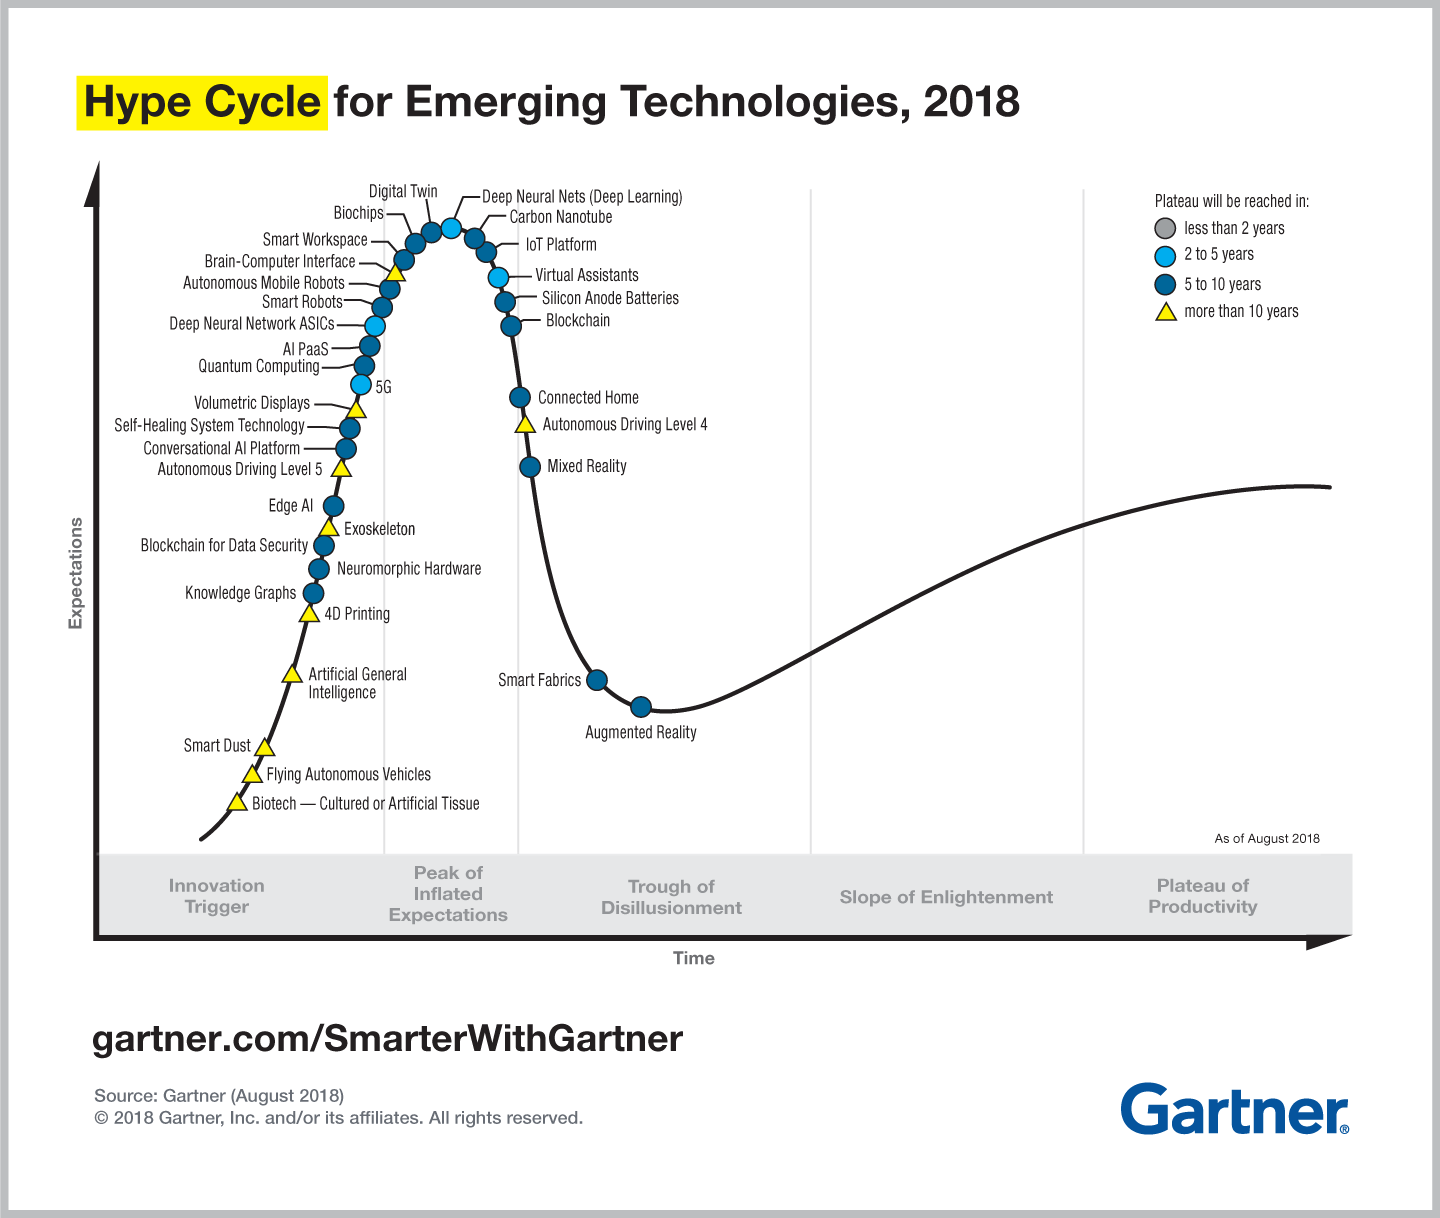
\includegraphics[width=0.7\textwidth]{PR_490866_5_Trends_in_the_Emerging_Tech_Hype_Cycle_2018_Hype_Cycle.png} 
                \caption{Gartner report of emerging technologies 2018}\label{gartner-2018}
            \end{figure}

            It is important to note though that as of 2018, it'll still take more than 10 years to reach a plateau of productivity.
            Although there is no mention about this technology in subsequent reports in the following year, two market revenue forecasts from 2015 until 2022 and 2018 until 2022 show a similar pattern in figure \ref*{statista-revenue}.

            \begin{figure}[h]
                \centering
                \subfloat[\centering \cite{Statista.24052021b}]{{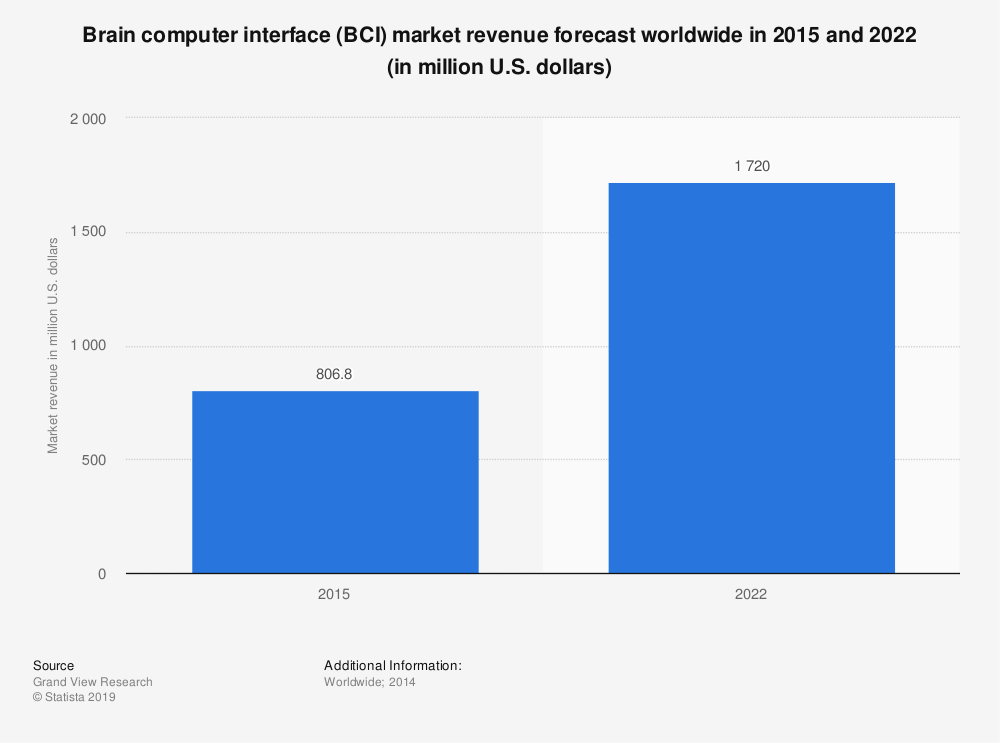
\includegraphics[width=0.49\textwidth]{statistic_id1015039_brain-computer-interface-market-value-worldwide-2015-and-2022.png} }}%
                %\qquad
                \subfloat[\centering \cite{Statista.24052021}]{{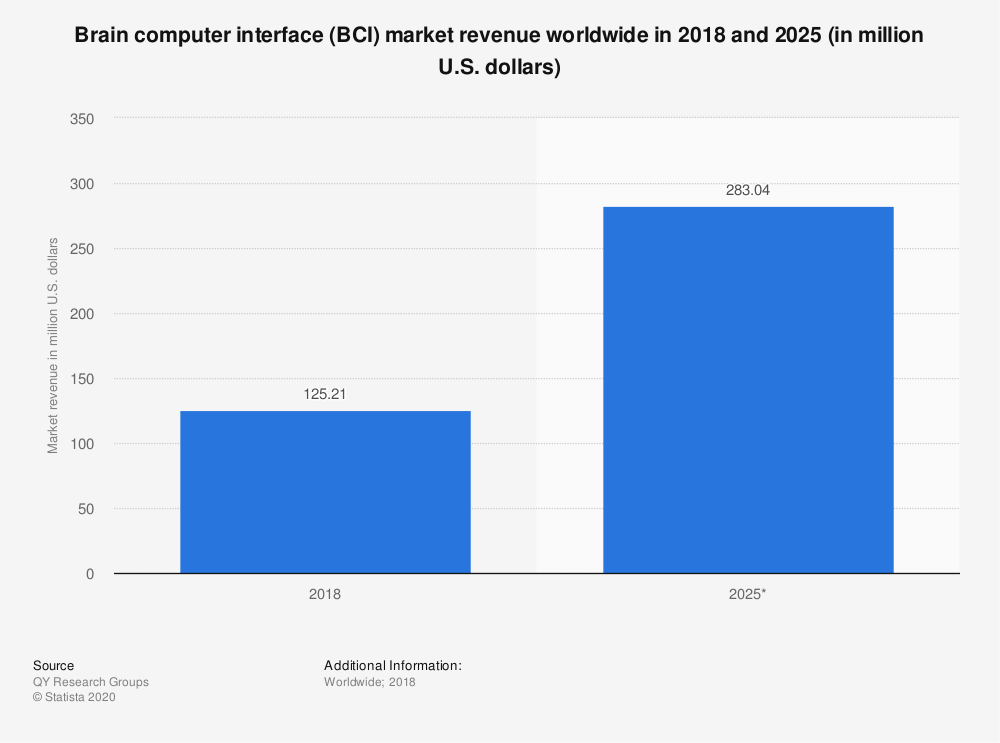
\includegraphics[width=0.49\textwidth]{statistic_id1015013_brain-computer-interface-market-value-worldwide-2018-and-2025.png}}}%
                \caption{Statista revenue forecast as of 2015 and 2018}%
                \label{statista-revenue}
            \end{figure}        

            Essentially the market revenue expectation has been very inflated from 2015 on so that it was corrected downwards in 2018. But although the absolutes growth was projected to only a small fraction, the relative growth potential stayed about the same of doubling within the next seven years. This is very indicative for the technology being overhyped, as Gartner explains: (\cite{Gartner.24052021})

            \medskip
                \emph{A wave of “buzz” builds and the expectations for this innovation rise above the current reality of its capabilities. In some cases, an investment bubble forms, as happened with the web and social media}
            \medskip

            Nevertheless, what this technology sets apart from other featured technologies is the fact that is has been around for a few decades and has been continously researched upon. A strong indicator is the amount of organizations and conferences held about this entire discipline, as can be seen in section \ref*{related-work}. The fact that is has only been on the radar of early adopters and tech-enthusiasts in conjuction with market revenue projections is a strong indicator that this technology has reached a level of maturity which makes a widespread application outside of laboratories somewhat feasible.

            The latest \textit{2020 Gartner Hype Cycle} report shows already the enhanced version of bidirectional BCIs (titled \textit{"2-Way Brain Machine Interface"}) on the slope of innovation:

            \begin{figure}[h]     % h=here, t=top, b=bottom, p=page
                \centering
                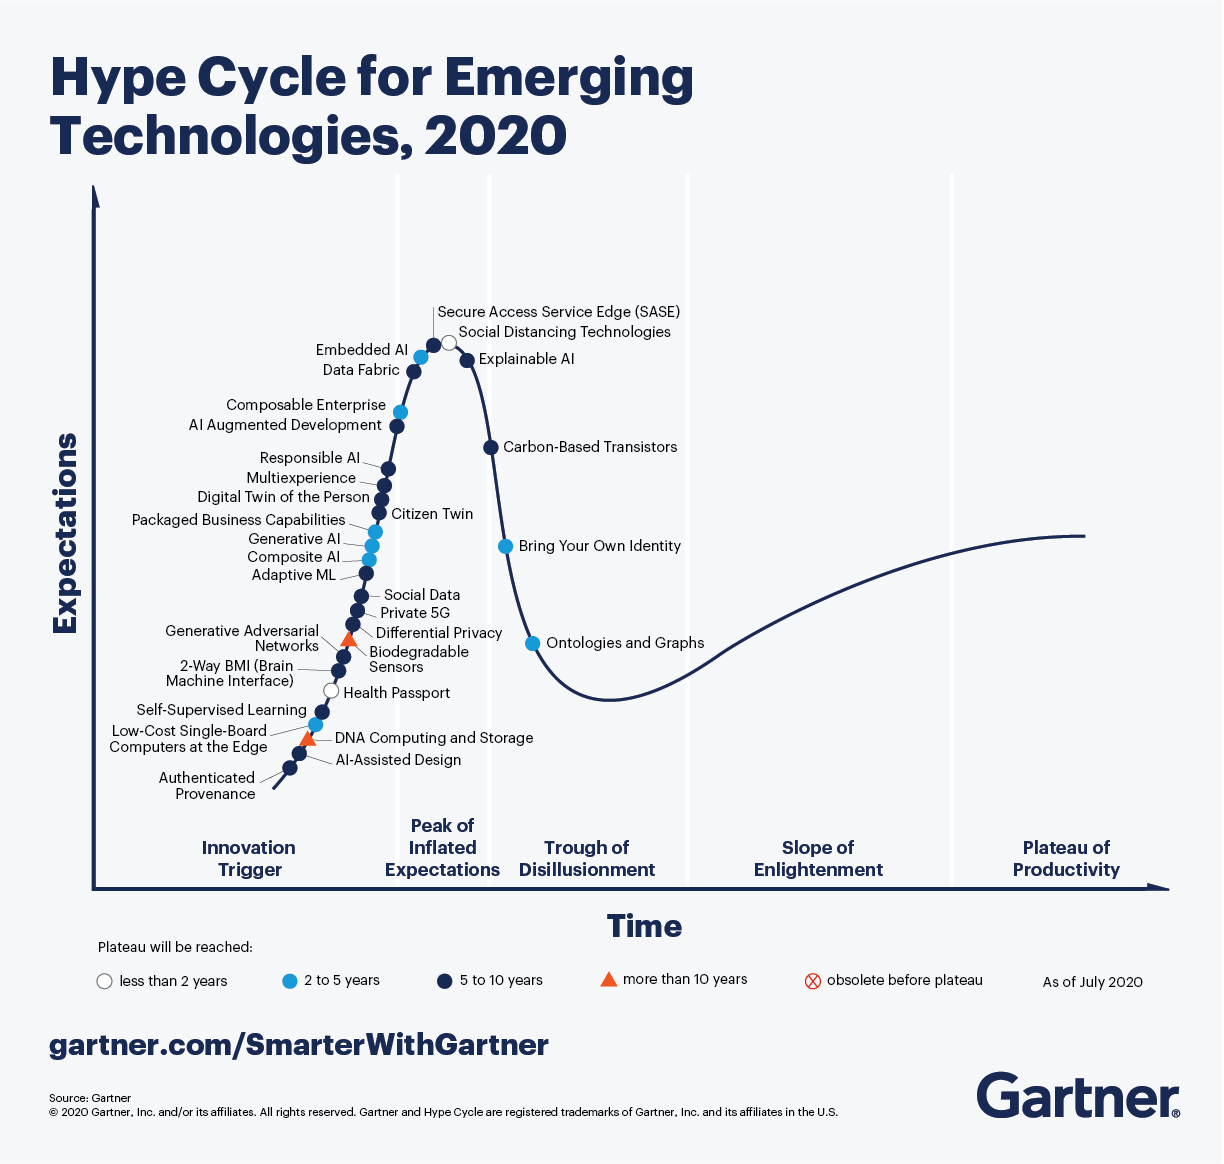
\includegraphics[width=0.8\textwidth]{gartner-hc-emerging-2020.png} 
                \caption{Gartner report of emerging technologies 2020}\label{gartner-2020}
            \end{figure}

            All in all, there are strong indicators that the technology gained traction over the last few years and could be considered a worthwile investment if approached with care.

        \section{Brain-Computer-Interfaces}\label{intro-bci}

            In this section a general overview of the working principle of these interfaces will be provided. Since this study is aimed at computer science and HCI\footnote{Human Computer Interaction}, the neuroscience and medical domain will be only covered very briefly.

            %https://www.frontiersin.org/articles/10.3389/fnins.2016.00295/full

            First studies began by \cite{Vidal.1973}, who investigated the possibility to use EEG\footnote{Electroencephalogram} waves, which were first recorded by \cite{Berger.1929}, as a way to create a direct interaction between a machine and a human brain. 

            There are three types of BCIs: invasive, partially invasive and non invasive. This depicts the degree of intrusion into the skull and brain tissue. \textit{Invasive} BCIs are electrodes, which are implanted directly into or onto the grey matter of the brain. This can cause long term issues like scars and also degraded singal strength according to \cite{Abdulkader.2015}. 
            Partially invasive BCI however are although located within the skull not in direct contact with the grey matter.
            Non-Invasive BCI are only placed on the head without intrusion of any tissue.
            Due to the direct contact, invasive BCI provide the best resolution of the measured signals. Non-invasive BCI in comparison suffer from signal degradation and deformation of the cranial bone tissue. 
            Therefore partially invasive BCI are a compromise between good signal strength and the risk of medical conditions.
            Another potential advantage of non-invasive BCIs is that these Interfaces could be easier mass-produced and become affordable to consumers. Also they don't require specialized medical knowledge and equipment to operate.

            The way these interfaces work is based on the same principle: A human brain emits electrical signals, which can be picked up.
            According to \cite{Vidal.1973}, they can be described as follows:

            \medskip
            \emph{"Embedded in this sustained "spontaneous" or "ongoing" electrical activity, short, distinctive (0.5-2 sec) waveforms can be found that are evoked, for instance, when a brief sensory message (stimulus) such as a brief illumination of the visual field or a tap on the forearm is received by the subject."}
            \medskip

            Based on the origin within the brain, these can be correlated to certain stimuli, mental and emotional states (\cite{JardimGoncalves.2018}) and according to \cite{Waldert.2016} been used to drive \emph{an external effector or affecting internal body parts and functions.} The external effector is the use case which is being examined in this study.

            Without a BCI, interaction with a computer requires some physical interaction with devices such as keyboards, mouses or gestures on a touch screen. There are mainly two different reasons, why these devices are a constraint to speed and efficiency of HCI. The first reason is a limitation on interaction speed: Although there is no definitive concensus about the speed of thinking, alone being able to type along the spoken word is unattainable for non-professional typists. A professional typist has to be able to type at 180 - 220 WPM\footnote{Words Per Minute} according to \cite{NCRA.25052021}. \cite{ScienceDaily.25052021} made a survey with 168.000 volunteers, where the fastest typists weren't even able to come close to this mark with 120 WPM. Therefore it is safe to assumt that typing in the same speed as thinking is impossible except for rare individuals who devoted a significant time practicing. Secondly: in applications such as games, where reaction time and accuracy is the fundamental element for success or failure, an interaction based on motoric interaction with a physical pointing device has some significant drawbacks like limited accuracy, if the whole chain of wrist movement in conjunction with a mouse is under scrutiny. 

            If a BCI was to replace these types interaction, these constraints could potentially be alleviated and interaction based on physical interaction rendered obsolete. 

        \section{Working principle}\label{working-principle}         

            Before any deeper considerations in regard to the general scope of this study can be made, it is important to understand the working principle of the BCI, which will be used. Although the vendor of the BCI in question does not disclose any details of the inner workings itself, it is safe to assume that the underlying technique used is the so called \textit{Steady State Visually Evoked Potential} - SSVEP in short. \cite{Sokol.1976} provides detailed inside into the topic from a neuroscientific point of view. The general principle however is that any visual stimuli cause a certain pattern of waves within the visual cortex of the brain. These patterns can be used to evaluate if a certain pattern is being seen \textit{and} in fokus of the person. 
            
            \begin{figure}[h]     % h=here, t=top, b=bottom, p=page
                \centering
                
\includegraphics[width=0.8\textwidth]{placeholder.jpg} 
                \caption{How VEP works in principle \todo{citation?}}\label{vep-principle}
            \end{figure}            
            
            This is being done by subsequently feeding the sensor data through a trained neural network. The objects, which are being seen by the person, have been labeled \textit{neurotags} (\cite{NextMind.23112020}) from the vendor of the BCI. These neurotags can provide two different readouts: If it is triggered (i.E. \textit{seen}) and the confidence, which depicts the level of \textit{focus} of the user on the neurotag (\cite{NextMind.18112020}).
            
            \begin{figure}[h]     % h=here, t=top, b=bottom, p=page
                \centering
                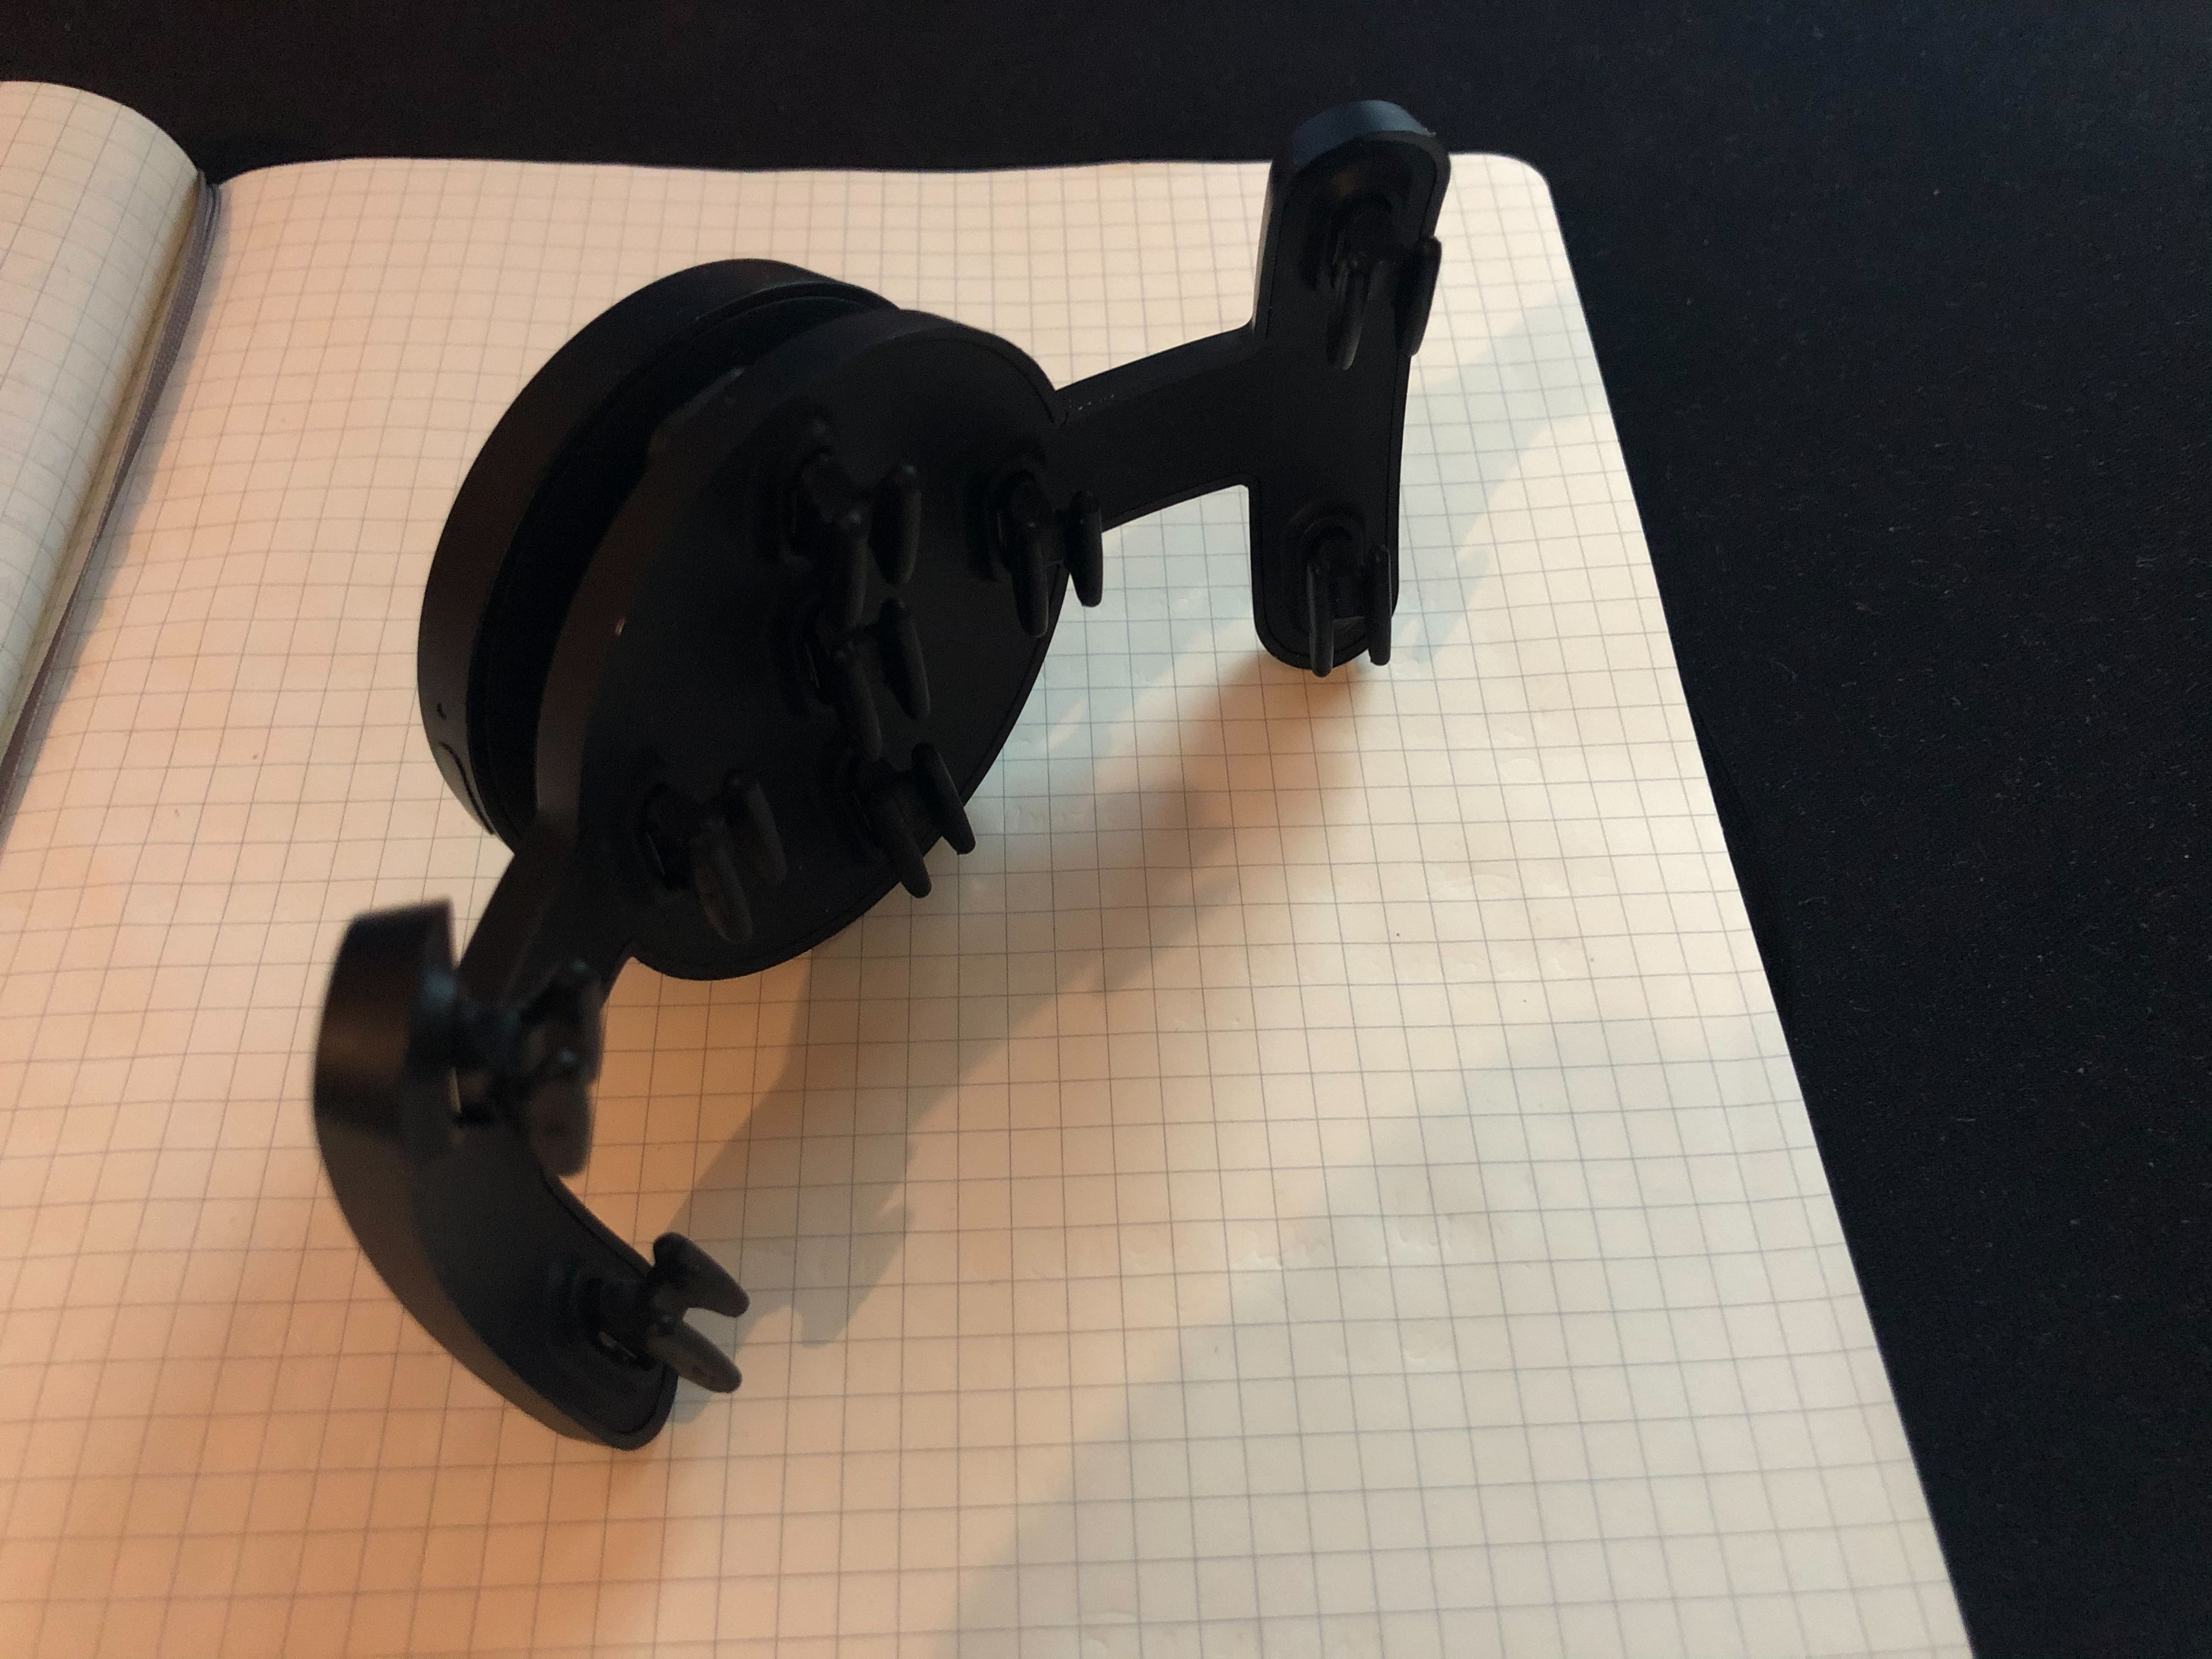
\includegraphics[width=0.8\textwidth]{electrodes-sensor} 
                \caption{Physical layout of the sensor}\label{electrodes-sensor}
            \end{figure}
            
            The physical layout of the sensor is show at figure \ref*{electrodes-sensor}. It has 18 eletrodes, which are arragend in pairs to cover the area, where the visual cortex is located at on the back of the cranium. It is battery driven and communicates via the Bluetooth LowEnergy protocol.

        \section{Related work}\label{related-work}

            As previously mentioned in section \ref*{introduction}, research on BCIs is partitioned between four different domains: \textit{medical engineering, neuroscience, computer science and HCI}. Apart from commercial entities such as \textit{Microsoft} or \textit{IBM} and scientific journals, the majority of the research community is clustered in three organizations: 

            \begin{itemize}
                \item ICBCI (\textit{International Conference of Brain Computer Interfaces}), which is a department of the WASET (\textit{World Academy of Science Engineering and Technology})
                \item EMBS (\textit{Engineering in Medicine and Biology Society}), which is a department of the IEEE
                \item BCI Society, which is an entity of its own
            \end{itemize}

            \medskip

            \emph{There are also research efforts in the east-asian region, according to corresponding tech-sites such as \cite{GlobalTimes.20042021} and \cite{TechwireAsia.24052021} but due to a language barrier, these sources cannot be considered.}

            \medskip

            To narrow the scope, where this research paper is located at, the considerations from section \ref*{use-case} are taken into accout. As already established in section \ref*{working-principle}, the sensor used in this study uses SSVEP and is non-invasive in nature. Therefore the general scope of this research is located in the realm of \textit{non-invasive BCI based on SSVEP used for HCI}.

            \medskip

            \cite{Oralhan.2016} and \cite{Resalat.2011} investigated the effects of different twinkle frequencies and duty cycles on the efficiency on precision of SSVEP BCI. They found that a certain combination of these parametres on fact could improve the ITR\footnote{Information Transfer Rate}. \cite{Lee.2016} used a similar approach and found the ideal combination in conjuction with Korean characters.
            \cite{S.M.Abdullah.2014} used a consumer ready BCI by \textit{EMOTIV} to create a \textit{Matrix-Speller} in the Bengali-Language to allow people who have lost the ability to communicate to express themselves again. 
            \cite{Chen.2020} also used a SSVEP BCI to implement a BCI-speller and scrutinized the tradeoff between responsiveness and accuracy.
            \cite{Chen.2020} designed an interface which is operated by a SSVEP BCI to control a robot arm, wich could administer food to disabled people.
            \cite{Soroush.2018} developed a SSVEP BCI which overcomes the necessity for training the sensor to the user who wears it. The prototype reached a similar precision as \textit{trained} interfaces.
            \cite{Gergondet.2015} investigated and selected certain visual stimuli which work best with certain use cases.
            \cite{Merino.2017} made a study, where participants controlled a UAV by using a SSVEP.
            \cite{Peters.2018} used simulated impairments to examine if usage of a SSVEP is still possible with medical conditions which affects speech and ocular impairments.

            Although not strictly within the SSVEP domain, the study by \cite{Beveridge.2017} showed very promising results by not using visual stimuli but mechanical ones, where he had teenagers playing a racing videogame with the aid of mechanical stimuli.

            There is a massive ongoing research effort to make the life of people who are suffering under ALS\footnote{Amyotrophic lateral sclerosis} better and improve their ability to communiate normally, by using SSVEP, a hybrid between an SSVEP and P300\footnote{An Event Related Potential (ERP) BCI} or purely P300 based BCI. A significant number of relevant studies has been published in the BCI Society Journal: \cite{Sugata.2016}, \cite{Holz.2015}, \cite{Speier.2017}, \cite{Geronimo.2017}, \cite{Speier.2018}, \cite{Mowla.2017}, \cite{Huggins.2016}. All these studies aimed to provide a better understanding and performance of using BCI on people with medical conditions, which imply serious physival impairments.


        \section{Use case "Neural Interface in VR"}\label{use-case}

            Before any use case can be conceived, it has to be determined what kind of interaction this interface allows. Section \ref*{intro-bci} covered briefly the concept of input taxonomies to elaborate optimization potentials with BCIs. According to \todo{Find some source} an input taxonomy depicts the DOF\footnote{Dimensions Of Freedom} and the granularity and magnitudes in regard to the interface which this interface offers.

            \begin{figure}[h]     % h=here, t=top, b=bottom, p=page
                \centering
                
\includegraphics[width=0.8\textwidth]{placeholder.jpg} 
                \caption{Taxonomy of the nextmind BCI. \todo{Todo: Create taxo schema}}\label{bci-taxonomy}
            \end{figure}

            Figure \ref*{bci-taxonomy} shows the input taxonomy of the BCI in question. It is derived from the API\footnote{Application Programming Interface} endpoints which the the SDK\footnote{Software Development Kit} of the sensor offers: \cite{NextMind.18112020}
            . The only two \textit{tracking resuls} are \textit{hit} and \textit{confidence}. Where hit is a two state interaction: the neurotag is being seen by the user and subsequently recognized by the sensor and its backend or it is not. The confidence property depicts the attention which the user is paying to the \textit{neurotag}. This is a continuous decimal value between 0 and 1.
            The fact that these types of interaction are based on neural activity raises the question if a pure mapping of continuous and discrete input modalities to established interfaces would be beneficial to the user experience. Under the reasonable assumption that without any training the metric \textit{focus} can only be deliberately controlled on a very coarse level, the necessary sensitiveness required for modern GUIs can not be achieved with this particular sensor. The remaining two state property, which can be utilized to select or deselect certain objects also only allows for limited interaction. However, these neurotags can be placed in arbitrary places. Although a \textit{toggle}-like behavior is not mentioned explicitly, it might be possible to de-select any activated neurotag when the \textit{focus} property falls under a certain value.

            \bigskip

            Based on the previous reasoning, the following questions can be raised in regard to the feasibility of any interface which could potententially be conceived with this technology:

            \begin{itemize}
                \item How fast is the perceived and measured reaction time of these neurotags?
                \item What is the minimum size the neurotags have to have in order to be recognizable?
                \item Is the interface usable for brains of all ages or do gerontological effects have an effect on usability?
                \item Do certain medical conditions (i.e. attentiveness disorder) have an impact on the usability?
                \item How fast can a user switch between neurotags?
                \item Is a BCI controlled GUI intuitive to use?
                \item Does a personal affinity to technology have an influence on the perceived difficulty of interaction?
            \end{itemize}

            These questions can be clustered into two groups: \textit{neurological} and \textit{interaction}. Although these considerations open up a vast space of potential cases. Therefore the priority is to examine wheter these interfaces are generally usable by the majority of users and if these interfaces are intuitive to use. 

        \section{Hypothesis}

            The considerations in the previous section leads to these two hypothesis:

            \medskip
            \emph{"Age does not have a detrimental effect on the ability to use a non-invasive BCI based on VEP technology."}
            \medskip

            and

            \medskip
            \emph{"VEP BCI operated GUIs are intuitive to use."}
            \medskip

    \chapter{Technological challenges}

        Due to being non-invasive there must exist certain drawbacks with this technology. I want to examine the shortcomings and possible ways to overcome these.    
        A valuable resource of information might be nextminds homepage.

        \section{Resolution of the Interface}

            %probablby make use of: https://www.tandfonline.com/doi/full/10.1080/2326263X.2018.1550710

            \begin{itemize}
                \item definition of the resolution parameter
                \item ITR
                \item accuracy
                \item input taxonomy diagram
                \item how to examine with survey                                     
            \end{itemize}

        \section{Constraints}

            As far as I understood, the interface allows for four different interaction goals. It would be interesting to see, which kinds of interaction are possible.                

            \begin{itemize}
                \item Interaction objects
                \item interaction types in regard to input taxonomy
                \item evaluation in user survey
            \end{itemize}

    \chapter{Survey Structure and layout}

        Before any survey can be designed, certain considerations like sample size, population ... \todo{ref to döring/bortz for details}
        have to be taken into account. Also depending on the desired outcome of the survey, the questionnaire has to be defined.

        \section{Considerations}

            \begin{itemize}
                \item what are my tools
                \item how to I operationalize the values for context
                \item What are my performance indicators
                \item Quantitative sampling to prove hypothesis
                \item gender equal
                \item 
            \end{itemize}

        \section{Survey structure}

            Based on the findings, I want to define the survey in this section.

            \begin{itemize}
                \item item 1
                \item ...
            \end{itemize}

        \section{Survey}

            How is the survey carried out. This depends largely on the outcome of section survey structure.

            \begin{itemize}
                \item item 1
                \item ...
            \end{itemize}

    \chapter{Survey results}

        Once the study has been structured and carried out, I can write down the results.

    \chapter{Findings}

        This section also depends on the outcomes in context to the resarch question.

    \chapter{Conclusion}

        \section{Results}

            Summarizing the results and findings of the study briefly.

        \section{Future Work}

            % might be a good suggestion to work on the shortcomings
            % https://www.tandfonline.com/doi/full/10.1080/2326263X.2020.1729652

            Based on the findings and new devices on the horizon, this should give a brief outlook on how to continue this research.

    \chapter{Acknowledgements}

        ...

    \appendix

        \chapter{Material}

            \section{Surveys, Protocols, etc.}

                Neque porro quisquam est qui dolorem ipsum quia dolor sit amet, consectetur, adipisci velit...

        %--------------------- VERZEICHNISSE ----------------

        \listoffigures % Abbildungsverzeichnis erzeugen
        \listoftables % Tabellenverzeichnis erzeugen

    %--------------------- LITERATURLISTE ---------------
    % Die Einträge sollen alphabetisch sortiert sein.

    \bibliography{references} 
    \bibliographystyle{unsrtnat}

    %--------------------- EIGENSTÄNDIGKEITSERKLÄRUNG ---------------
    \clearpage\thispagestyle{empty}
    \eigen  % im header definiert
    %--------------------------------------- ENDE ------------------------------------

\end{document}